\documentclass[conference]{IEEEtran}
\IEEEoverridecommandlockouts
\usepackage{cite}
\usepackage{amsmath,amssymb,amsfonts}
\usepackage{graphicx}
\usepackage{booktabs}
\usepackage{textcomp}
\usepackage{xcolor}
\usepackage{url}
\usepackage[colorlinks=true,linkcolor=blue!70!black,citecolor=blue!70!black,urlcolor=blue!70!black]{hyperref}

% ---------------------------------------------------------------- helpers
\newcommand{\TODO}[1]{\textcolor{red}{\textbf{[TODO: #1]}}}
\newcommand{\gen}[1]{\IfFileExists{generated/#1.tex}{\input{generated/#1.tex}}{\TODO{missing \detokenize{generated/#1.tex}; run genai.report\_assets}}}
% figure that shows a red placeholder if the image file does not exist yet
\newcommand{\optfig}[4]{% file, width, caption, label
  \begin{figure}[t]\centering
  \IfFileExists{figures/#1}{\includegraphics[width=#2]{figures/#1}}{\fbox{\parbox{0.9\columnwidth}{\TODO{figure \detokenize{#1} missing}}}}
  \caption{#3}\label{#4}\end{figure}}
\newcommand{\optfigw}[4]{% wide (two column) version
  \begin{figure*}[t]\centering
  \IfFileExists{figures/#1}{\includegraphics[width=#2]{figures/#1}}{\fbox{\parbox{0.9\textwidth}{\TODO{figure \detokenize{#1} missing}}}}
  \caption{#3}\label{#4}\end{figure*}}

\newcommand{\optpair}[4]{% two images side by side: file1, file2, caption, label
  \begin{figure*}[t]\centering
  \IfFileExists{figures/#1}{\includegraphics[width=0.38\textwidth]{figures/#1}}{\fbox{\TODO{#1 missing}}}\hfill
  \IfFileExists{figures/#2}{\includegraphics[width=0.58\textwidth]{figures/#2}}{\fbox{\TODO{#2 missing}}}
  \caption{#3}\label{#4}\end{figure*}}

\definecolor{hlsec}{RGB}{255,236,153}
\definecolor{hlsub}{RGB}{255,246,201}
\definecolor{hllink}{RGB}{255,230,0}
\let\oldsection\section
\renewcommand{\section}[1]{\oldsection{\textbf{#1}}}
\let\oldsubsection\subsection
\renewcommand{\subsection}[1]{\oldsubsection{\textbf{#1}}}
\newcommand{\hlurl}[1]{\colorbox{hllink}{\strut\url{#1}}}

\begin{document}

\title{Image Restoration with Universal, Hard-Routed and Soft Mixture-of-Experts Autoencoders and Style-Conditioned Face-to-Sketch Generation with a Conditional GAN}

\author{\IEEEauthorblockN{Iman Suleman}
\IEEEauthorblockA{Roll No.\ 23i-0618, Section CS-G\\
Department of Computer Science, FAST NUCES Islamabad\\
Generative AI, Assignment 1}}

\maketitle

\begin{abstract}
This report covers four related models I built for the Generative AI course. The first three restore Oxford-IIIT Pet images damaged by salt-and-pepper noise, Gaussian blur or black rectangles: one universal denoising autoencoder, a classifier that sends each image to one of three specialist autoencoders, and a soft mixture-of-experts whose gate starts from that classifier. The fourth is a conditional GAN that turns a face photo into a sketch in one of three FS2K styles. All models were tuned with Optuna, tracked with MLflow and exported to ONNX, where the outputs match PyTorch to within $2.1\times10^{-6}$. They run together in one React and FastAPI app started with Docker Compose. On the fixed test set the soft mixture-of-experts is best on single corruptions, with a mean PSNR of 24.22\,dB against 23.63\,dB for the universal autoencoder and 23.33\,dB for hard routing. When two corruptions are applied at once the universal autoencoder wins (19.42\,dB against 19.07 and 18.88\,dB). The classifier is 99.9\% accurate. The cGAN reaches PSNR 15.61\,dB and SSIM 0.538, compared with 6.73\,dB and 0.289 for using the grayscale photo as the sketch.
\end{abstract}

\begin{IEEEkeywords}
denoising autoencoder, mixture of experts, image restoration, conditional GAN, Optuna, ONNX
\end{IEEEkeywords}

% =============================================================================
\section{Introduction}
Real photos rarely come with a label saying what is wrong with them. A restoration system can deal with this in three ways: train one model for every kind of damage, detect the damage and call a specialist, or blend several specialists with learned weights. Tasks 1 to 3 compare these three options under the same conditions: the same data split, the same runtime corruption code, the same fixed test set and the same metrics. Task 4 is a different problem. It translates a photo into a sketch, and a style label has to control the output.

The report contains a corruption pipeline that can be reproduced, with fixed validation and test sets (Section~\ref{sec:data}); a comparison of universal, hard-routed and soft-routed restoration, including oracle versus predicted routing and a test with two corruptions at once (Sections~\ref{sec:method} and~\ref{sec:results}); a pix2pix-style GAN where the style enters both the generator and the discriminator; Optuna studies for every model; and a containerised app for all four tasks (Section~\ref{sec:app}). The code and the demo video are listed in the next section.

% =============================================================================
\section{Project Links}
\begin{itemize}
\item \textbf{Code repository (GitHub):} \url{https://github.com/ImaanSuleiman/genai-assignment1}
\item \textbf{Demo video (YouTube):} \url{https://youtu.be/KFsUBjwYsj8}
\end{itemize}

% =============================================================================
\section{Related Research and Design Decisions}\label{sec:related}
\textbf{Denoising autoencoders.} Vincent et al.\ showed that training an autoencoder to rebuild a clean image from a damaged one makes it learn structure instead of copying \cite{vincent2008}. DnCNN \cite{zhang2017dncnn} and context encoders \cite{pathak2016} showed that convolutional networks cope with noise and missing regions, and all-in-one restoration work \cite{li2022airnet} raises the question I study here: can one network for several kinds of damage compete with specialists? I kept a plain encoder, bottleneck, decoder shape with no unrestricted skip connections, as the assignment requires. A full skip would let the decoder copy the noisy input and defeat the bottleneck. One narrow skip is available as an option (\texttt{--limited-skip}) so its effect can be measured later.

\textbf{Loss functions.} L1 gives sharper restorations than L2, and the structural similarity index (SSIM) \cite{wang2004ssim} rewards local contrast and structure. I train with $\alpha\mathcal{L}_{L1}+(1-\alpha)(1-\mathrm{SSIM})$ and let Optuna pick $\alpha$. The validation objective $\mathrm{L1}+(1-\mathrm{SSIM})$ does not use $\alpha$. Otherwise the search would simply prefer whichever weight makes the objective numerically smallest.

\textbf{Mixtures of experts.} Adaptive mixtures of local experts \cite{jacobs1991} learn a gate that weights the experts' outputs, and sparsely gated layers \cite{shazeer2017} scale the idea up. Both report that one expert can end up receiving nearly everything unless the load is balanced. To avoid this in Task 3 I start the gate and experts from Task 2, warm up the gate with the experts frozen, use balanced batches and add the balance term $\sum_k(\bar w_k-\frac14)^2$. Optuna trials are pruned when routing collapses, meaning any mean weight above 0.7 or below 0.03.

\textbf{Conditional GANs.} The cGAN \cite{mirza2014} feeds side information to both networks. Pix2pix \cite{isola2017} adds a U-Net \cite{ronneberger2015} generator, a PatchGAN discriminator and an L1 term (weight 100) for paired translation. I follow that recipe at $128\times128$ with six down-sampling stages, so the bottleneck is $2\times2$. The style label is a learned embedding that goes in three places: it is added to the generator input as extra channels, it is injected into every decoder block with FiLM scale and shift \cite{perez2018film}, and it is added to the discriminator input. That makes it part of the model and not just a label in the interface. I use instance normalisation \cite{ulyanov2016} instead of batch normalisation because the batch sizes in the Optuna search are small.

Table~\ref{tab:decisions} lists the main design decisions and the evidence behind each.

\textbf{Hyper-parameter search.} Every model uses Optuna \cite{akiba2019} with the TPE sampler and median pruning. Studies are saved in SQLite so they can be resumed and inspected.

\begin{table}[t]
\centering\caption{Main design decisions and the evidence behind them.}\label{tab:decisions}
\footnotesize
\begin{tabular}{p{2.1cm}p{2.6cm}p{3.1cm}}
\toprule
Decision & Alternatives considered & Reason / evidence \\
\midrule
No unrestricted skips in UDAE & U-Net style skips & Skips copy corrupted input \cite{vincent2008}; ablation switch provided \\
L1 + SSIM loss & L2, L1 only & L1 sharper than L2; SSIM preserves structure \cite{wang2004ssim} \\
Spatial $8\times8$ latent & flat dense vector & Keeps spatial layout; dense layers over $128^2$ maps add parameters without benefit \\
Avg+max pooling classifier & avg pooling only & Max pooling keeps local evidence (isolated noise, mask edges) \\
Balanced batches & random class mix & Needed for unbiased classifier and for $\bar w_k$ in the balance loss \\
Gate init.\ from Task 2 & random gate & Avoids early expert collapse \cite{shazeer2017} \\
FiLM + input-channel style & label only in the UI & Assignment requires style inside $G$ and $D$ \\
Instance norm in GAN & batch norm & Small GAN batches make batch statistics unreliable \cite{ulyanov2016} \\
\bottomrule
\end{tabular}
\end{table}


% =============================================================================
\section{Datasets and Preprocessing}\label{sec:data}
\subsection{Oxford-IIIT Pet (Tasks 1--3)}
The Oxford-IIIT Pet dataset \cite{parkhi2012} has cat and dog photos from 37 breeds. I convert the official \texttt{trainval} images to RGB, resize them to $128\times128$ and split them 80/20 into training and validation sets with seed 42 (\gen{dataset_sizes} images). The official test images are not touched until the final evaluation. All three tasks share this split, and breed labels are never used.

\subsection{Runtime corruption pipeline}
Nothing corrupted is stored on disk. Every time a training image is loaded, one of four conditions is drawn with equal probability and a severity is sampled (Table~\ref{tab:corr}). The condition also serves as the label for the corruption classifier. Salt-and-pepper noise sets a pixel to black or white with equal chance. Blur is an OpenCV Gaussian blur with a kernel of 3, 5 or 7. Occlusion draws one to three black rectangles whose combined area covers 10 to 35\% of the image, at random positions.

\begin{table}[t]
\centering\caption{Corruption configuration.}\label{tab:corr}
\footnotesize
\begin{tabular}{p{1.5cm}p{3.0cm}p{2.9cm}}
\toprule
Condition & Training (sampled per load) & Test (fixed low/medium/high) \\
\midrule
Clean & original image & original image \\
Salt-and-pepper & $p\sim U(0.02,0.15)$ & $p\in\{0.03,0.08,0.15\}$ \\
Gaussian blur & $k\in\{3,5,7\}$, $\sigma\sim U(0.5,2.5)$ & $(k,\sigma)\in\{(3,0.7),(5,1.5),(7,2.5)\}$ \\
Occlusion & 1--3 rectangles, joint area 10--35\% & 1/2/3 rectangles, area $\approx$10/20/35\% \\
\bottomrule
\end{tabular}
\end{table}

Validation and test corruptions are fixed so results can be compared between runs. The validation manifest holds one balanced corruption per validation image. The test manifest holds the clean image plus three corruptions at three severities, ten entries per image. Both are generated once and saved as JSON, with the type, severity, mask coordinates, blur settings and random seed of every entry. For reporting, validation severities are grouped into low, medium and high using the tertiles of the training range.

\subsection{FS2K (Task 4)}
FS2K \cite{fan2022fs2k} has 2{,}104 paired photos and sketches in three styles. I use the official train and test split and hold out 15\% of the training part for validation, stratified by style with seed 42. Photos and sketches are resized to $128\times128$. Augmentation (a horizontal flip and a random crop resized back) draws one random transformation and applies it to both images of a pair, so the pairing stays correct.

% =============================================================================
\section{Methodology}\label{sec:method}
\subsection{Task 1: universal denoising autoencoder}
The UDAE (Fig.~\ref{fig:udae}) has four stride-2 encoder stages, a $1\times1$ convolution down to a latent tensor of $C\times8\times8$ values, and a decoder made of nearest-neighbour up-sampling and convolution blocks that ends in a sigmoid. With $C=16$ the latent has 1{,}024 numbers, 48 times fewer than the $3\times128\times128$ input, so the network cannot simply copy its input. It is trained with
\begin{equation}
\mathcal{L}_{UDAE}=\alpha\,\mathcal{L}_{L1}(x,\hat{x})+(1-\alpha)\bigl(1-\mathrm{SSIM}(x,\hat{x})\bigr),
\end{equation}
with $\hat{x}=D(E(\tilde{x}))$. The network is never told which corruption was applied.
\optfig{arch_udae.png}{0.95\columnwidth}{Architecture of the universal denoising autoencoder.}{fig:udae}

\subsection{Task 2: classifier and hard-routed specialists}
The classifier is a convolutional network whose channel widths were chosen by Optuna, with average and max global pooling. It is trained with cross-entropy on batches that hold exactly one quarter of each class. The three specialists (salt-and-pepper, blur, occlusion) share one architecture from a shared Optuna search, but they are trained separately, with different seeds and weights, each only on its own corruption and with the clean image as the target. At inference (Fig.~\ref{fig:hard} shows the pipeline)
\begin{equation}
\hat{x}=\begin{cases}\tilde{x}, & r=\text{clean}\\ A_{r}(\tilde{x}), & \text{otherwise}\end{cases},\quad r=\arg\max_k p_k,
\end{equation}
so clean images take an identity bypass. I evaluate two modes. Oracle routing uses the true label from the manifest and isolates the quality of the specialists. Predicted routing uses the classifier and measures the system as it would be deployed.
\optfig{arch_hard.png}{0.95\columnwidth}{Hard-routed restoration pipeline.}{fig:hard}

\subsection{Task 3: jointly trained soft mixture-of-experts}
The gate $G$ is the Task~2 classifier, and the experts are the three specialists plus an identity branch. With $w=\mathrm{softmax}(G(\tilde{x})/\tau)$ the output is $\hat{x}=w_0\tilde{x}+w_1A_{salt}(\tilde{x})+w_2A_{blur}(\tilde{x})+w_3A_{occ}(\tilde{x})$, which is differentiable in both the gate and the experts (Fig.~\ref{fig:soft}). Stage~A trains only the gate with the experts frozen (learning rate $3\eta$). Stage~B unfreezes everything and fine-tunes at learning rate $\eta$. The loss is
\begin{equation}
\mathcal{L}_{MoE}=\lambda_1\mathcal{L}_{L1}+\lambda_s(1-\mathrm{SSIM})+\lambda_c\mathcal{L}_{CE}+\lambda_b\sum_{k=0}^{3}\bigl(\bar w_k-\tfrac14\bigr)^2,
\end{equation}
where $\lambda_s=1-\lambda_1$, the cross-entropy uses the raw gate logits and the runtime corruption label, and $\bar w_k$ is the mean weight of branch $k$ in a class-balanced batch. I use the quadratic balance loss suggested in the assignment. It is smallest when the batch-mean weights are uniform, which is the right target because a balanced batch has 25\% of each condition.
\optfig{arch_soft.png}{0.95\columnwidth}{Soft mixture-of-experts model.}{fig:soft}

\subsection{Task 4: style-conditioned cGAN}
The generator is a six-stage U-Net with skip connections and style FiLM in every decoder block (Fig.~\ref{fig:cgan}). The discriminator is a PatchGAN over the photo, the sketch and the style embedding stacked together. The discriminator minimises $\tfrac12[\mathrm{BCE}(D(x,y,s),1)+\mathrm{BCE}(D(x,G(x,s),s),0)]$ and the generator minimises $\mathcal{L}_G=\mathcal{L}_{adv}+\lambda_{L1}\|y-G(x,s)\|_1$. Five loss terms (D-real, D-fake, G-adversarial, G-L1 and validation) are logged every epoch, and the same four validation photos are rendered in all three styles at fixed intervals (Fig.~\ref{fig:evolution}).
\optfig{arch_cgan.png}{0.95\columnwidth}{Conditional GAN architecture.}{fig:cgan}

% =============================================================================
\section{Hyper-parameter Optimisation}\label{sec:optuna}
Every model is tuned with an Optuna TPE study and median pruning. Studies are saved in SQLite, every trial is a nested MLflow run, and trials use a shorter epoch budget. The chosen configuration is then retrained for the full schedule. Table~\ref{tab:optuna} summarises the studies and Tables~\ref{tab:space_task1_udae}--\ref{tab:space_task4_cgan} list the search spaces. The Task~1 objective is validation $\mathrm{L1}+(1-\mathrm{SSIM})$ on the fixed validation manifest. The classifier maximises validation macro-F1. The specialist search averages the objective over the three specialists, so the shared architecture suits all of them. The MoE search uses the same objective as Task~1 and prunes collapsed routing. The GAN search uses L1+(1-SSIM) between the generated and the paired sketch on the validation set, with fewer epochs. That is only a proxy, because it rewards fidelity and not realism (see Section~\ref{sec:limits}).

\gen{optuna_summary}
\gen{space_task1_udae}
\gen{space_task2_classifier}
\gen{space_task2_specialists}
\gen{space_task3_moe}
\gen{space_task4_cgan}

\optpair{task1_udae_history.png}{task1_udae_importance.png}{Task 1 (UDAE) Optuna study: optimisation history (left) and hyper-parameter importance (right).}{fig:opt1}
\optpair{task2_classifier_history.png}{task2_classifier_importance.png}{Task 2 classifier study: optimisation history (left) and importance (right).}{fig:opt2c}
\optpair{task2_specialists_history.png}{task2_specialists_importance.png}{Task 2 specialist study (shared architecture): history (left) and importance (right).}{fig:opt2s}
\optpair{task3_moe_history.png}{task3_moe_importance.png}{Task 3 soft-MoE study: history (left) and importance (right).}{fig:opt3}
\optpair{task4_cgan_history.png}{task4_cgan_importance.png}{Task 4 cGAN study: history (left) and importance (right).}{fig:opt4}
Table~\ref{tab:optuna} and Figs.~\ref{fig:opt1}--\ref{fig:opt4} show how each search went and which settings mattered. The history plots show how much tuning gained. In Task~1 the best objective improved from 0.451 at the first trial to 0.412 at trial 12 and did not improve afterwards. The classifier barely moved (Fig.~\ref{fig:opt2c}): every finished trial scored a macro-F1 between 0.971 and 0.989, so tuning mattered little for that easy task. The specialist search gained the most, from 0.585 to 0.439 (Fig.~\ref{fig:opt2s}). The MoE search (Fig.~\ref{fig:opt3}) went from 0.210 to 0.191 and its best trial was one of the last, so with only 20 trials it probably had not converged. The GAN objective fell from 0.627 to 0.563. The importance plots rank the parameters. In Task~1 the loss weight $\alpha$ mattered most (importance 0.47), then the learning rate (0.18) and the base width and latent size (0.12 each). The chosen values were $\alpha=0.53$, latent $32\times8\times8$ and learning rate $2.6\times10^{-4}$. An $\alpha$ near 0.5 makes sense because the validation objective weighs L1 and $1-\mathrm{SSIM}$ equally, so the training loss that matches it works best. The 32-channel latent (2{,}048 values, 24 times smaller than the input) won over smaller ones, but latent size had low importance, so the search showed no strong preference. Only 12 of the 25 trials finished (13 were pruned), so these importance values are noisy.

For the classifier, dropout (0.54), learning rate (0.21) and weight decay (0.20) mattered most, and channel width hardly mattered (0.03). That fits an easy task: almost every finished trial passed 97\% validation accuracy, and the smallest network won. For the specialists, $\alpha$ (0.72) and the learning rate (0.25) dominated, and the chosen $\alpha=0.70$ favours L1 more than Task~1 did. For the MoE, the gate temperature (0.39), the balance weight (0.32) and the learning rate (0.22) mattered most, and a softer gate ($\tau=1.37$) was preferred. The cross-entropy weight mattered little (0.027).

For the GAN, the two learning rates (0.30 and 0.29), dropout (0.24) and $\lambda_{L1}$ (0.17) mattered, while style dimension, batch size and width had no measurable effect. The chosen $\lambda_{L1}\approx197$ is about twice the usual pix2pix value of 100. Only 10 of the 15 GAN trials finished, each of 10 epochs, and the objective is a fidelity proxy, so read its ranking with caution.

% =============================================================================
\section{Experimental Setup}
\subsection{Training procedure}
All models are written in PyTorch and were trained on a Google Colab runtime with an NVIDIA T4 GPU. I use Adam (AdamW for the classifier) with cosine learning-rate decay, and Adam with $\beta_1=0.5$ for the GAN. All seeds are 42. The tasks are trained in the order they depend on each other. First the UDAE (Task~1) trains for 60 epochs on images that are corrupted as they are loaded. Next the classifier trains for 40 epochs on class-balanced batches, and each of the three specialists trains for 40 epochs on its own corruption only. The soft MoE (Task~3) then starts from those weights and trains for 2 warm-up epochs (gate only) plus 30 joint epochs. The cGAN (Task~4) trains for 150 epochs with the discriminator and generator updated alternately. Before each full run, Optuna chose the hyper-parameters with shorter trials of 6 epochs (UDAE), 5 (classifier), 4 (specialists), 4 (MoE) and 10 (cGAN), and the chosen configuration was then retrained for the full schedule.

\subsection{Evaluation protocol}
Metrics are PSNR, SSIM and L1 against the clean target on the fixed test manifest. Task~2 also reports accuracy, macro precision, recall and F1, and a normalised confusion matrix. Hyper-parameters, per-epoch losses, checkpoints and sample images are tracked in MLflow, and Fig.~\ref{fig:mlflow} shows screenshots of its UI. Figs.~\ref{fig:mlflow} and~\ref{fig:mlflowexp} show that every task has its own experiment, with one parent run per Optuna study, one nested run per trial and one long run for the final training.
\begin{figure*}[t]
\centering
\IfFileExists{figures/mlflow_t1.png}{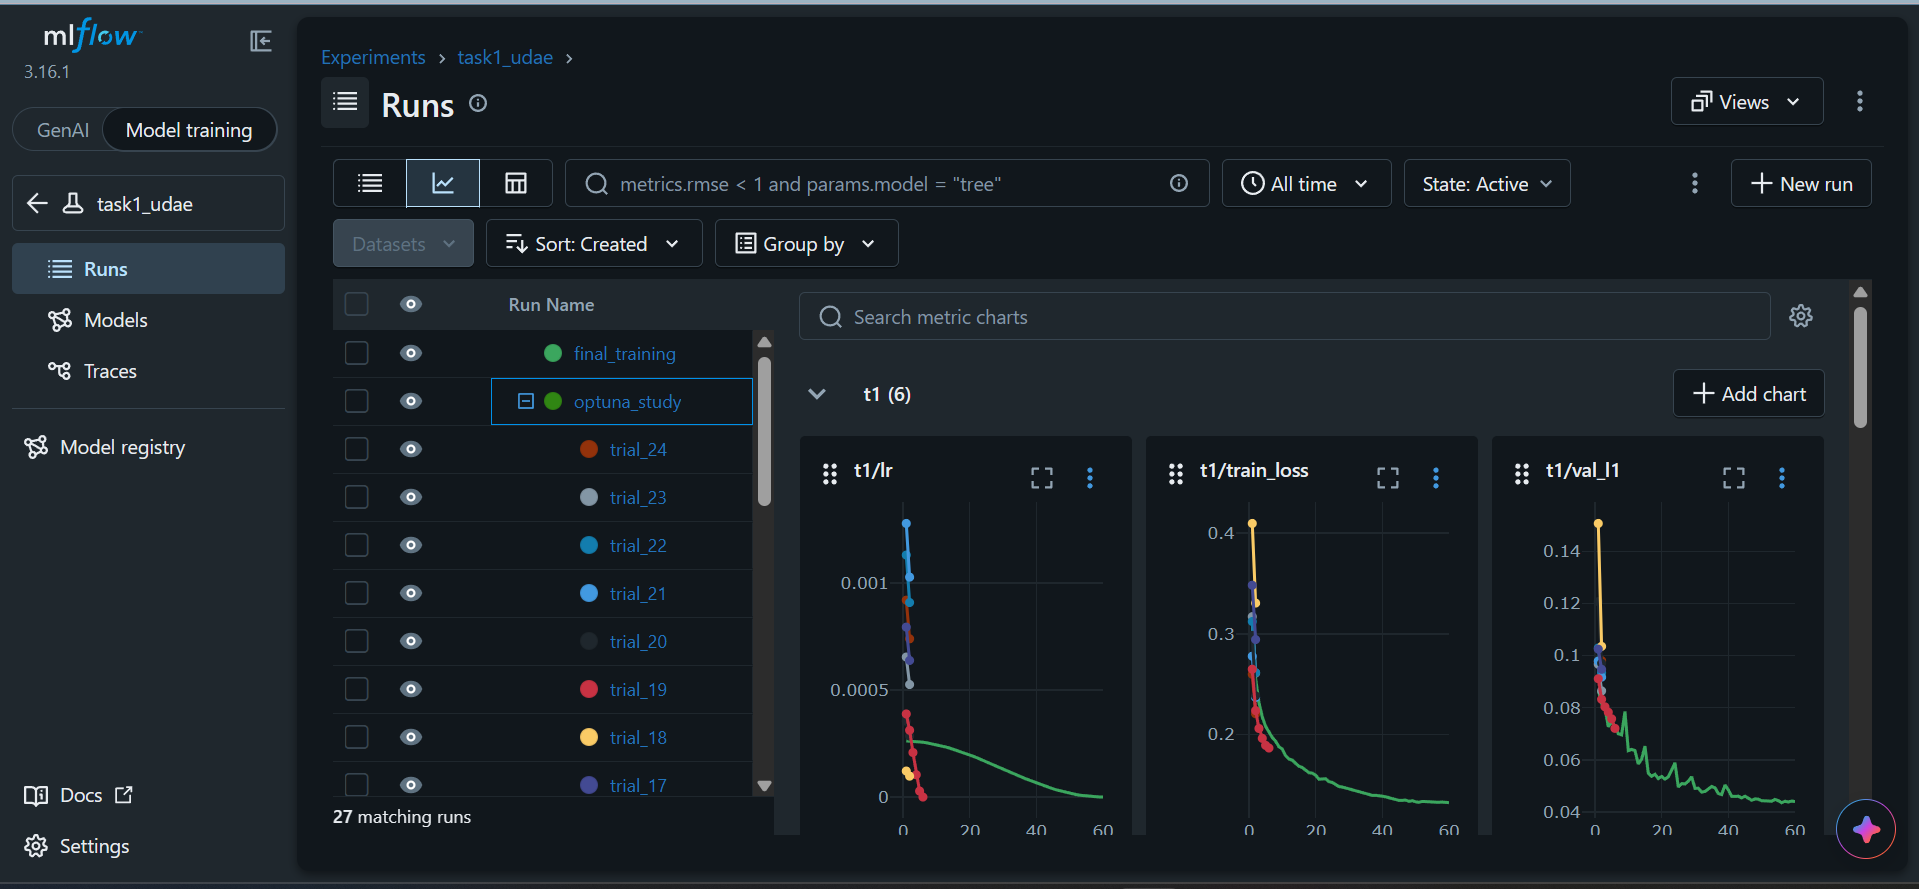
\includegraphics[width=0.49\textwidth]{figures/mlflow_t1.png}}{\fbox{\TODO{mlflow\_t1.png missing}}}\hfill
\IfFileExists{figures/mlflow_t2.png}{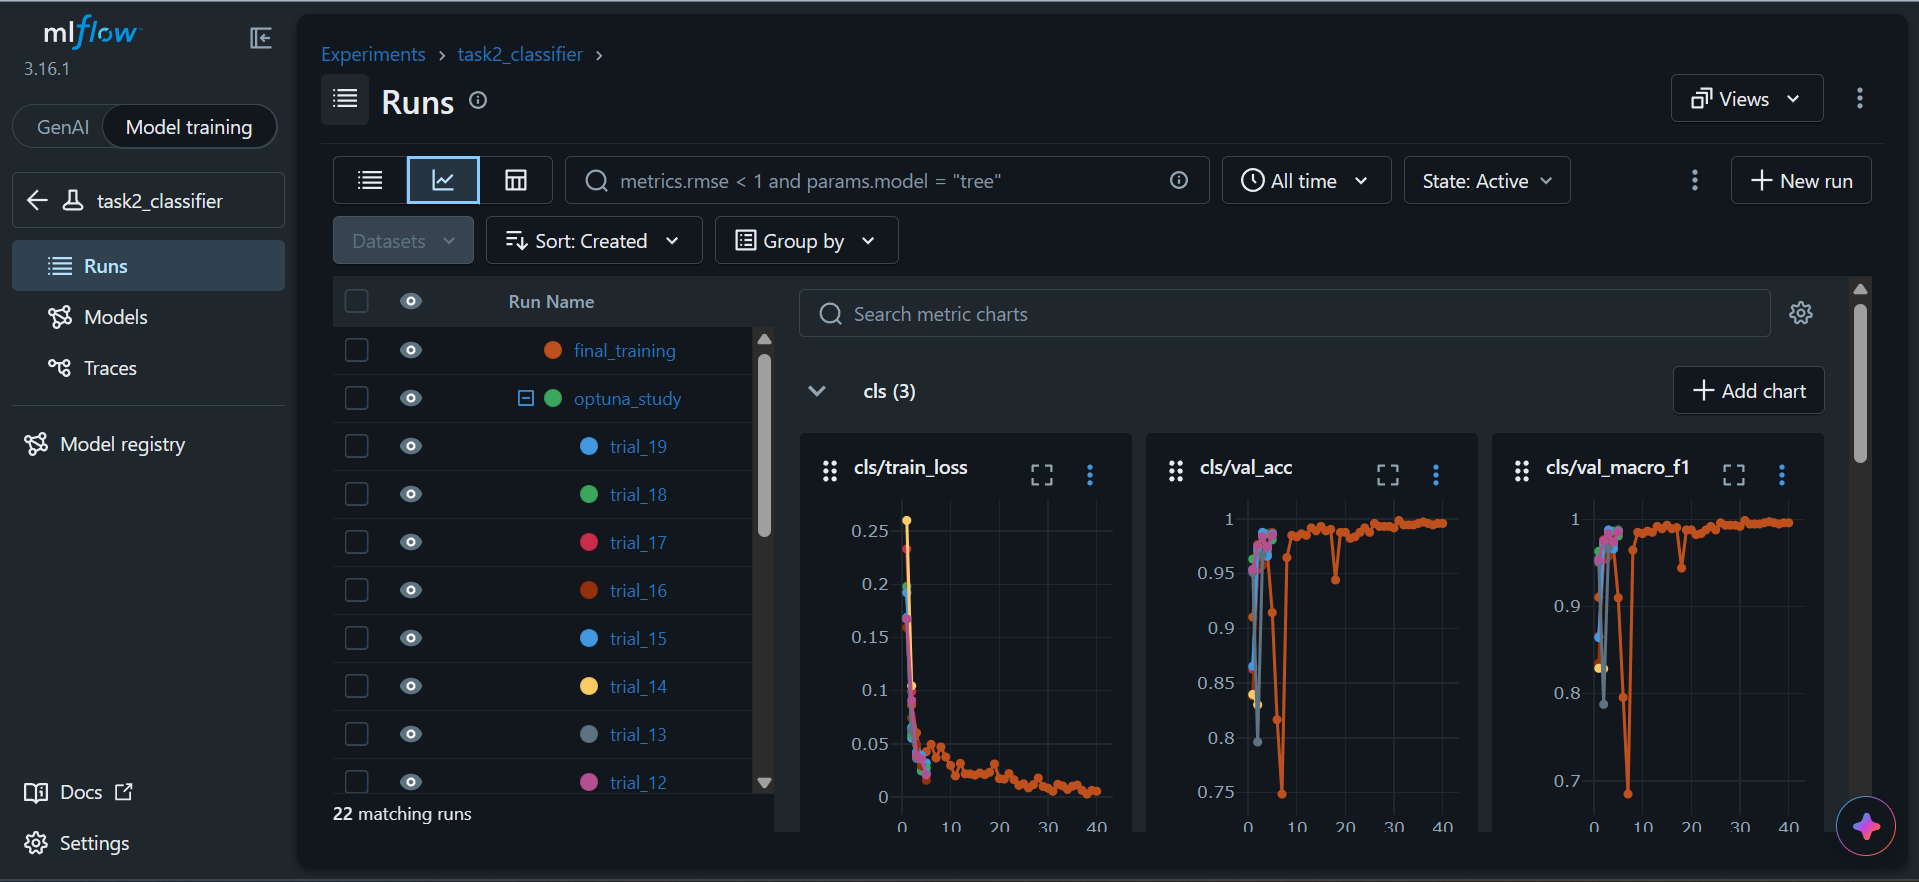
\includegraphics[width=0.49\textwidth]{figures/mlflow_t2.png}}{\fbox{\TODO{mlflow\_t2.png missing}}}\\[3pt]
\IfFileExists{figures/mlflow_t3.png}{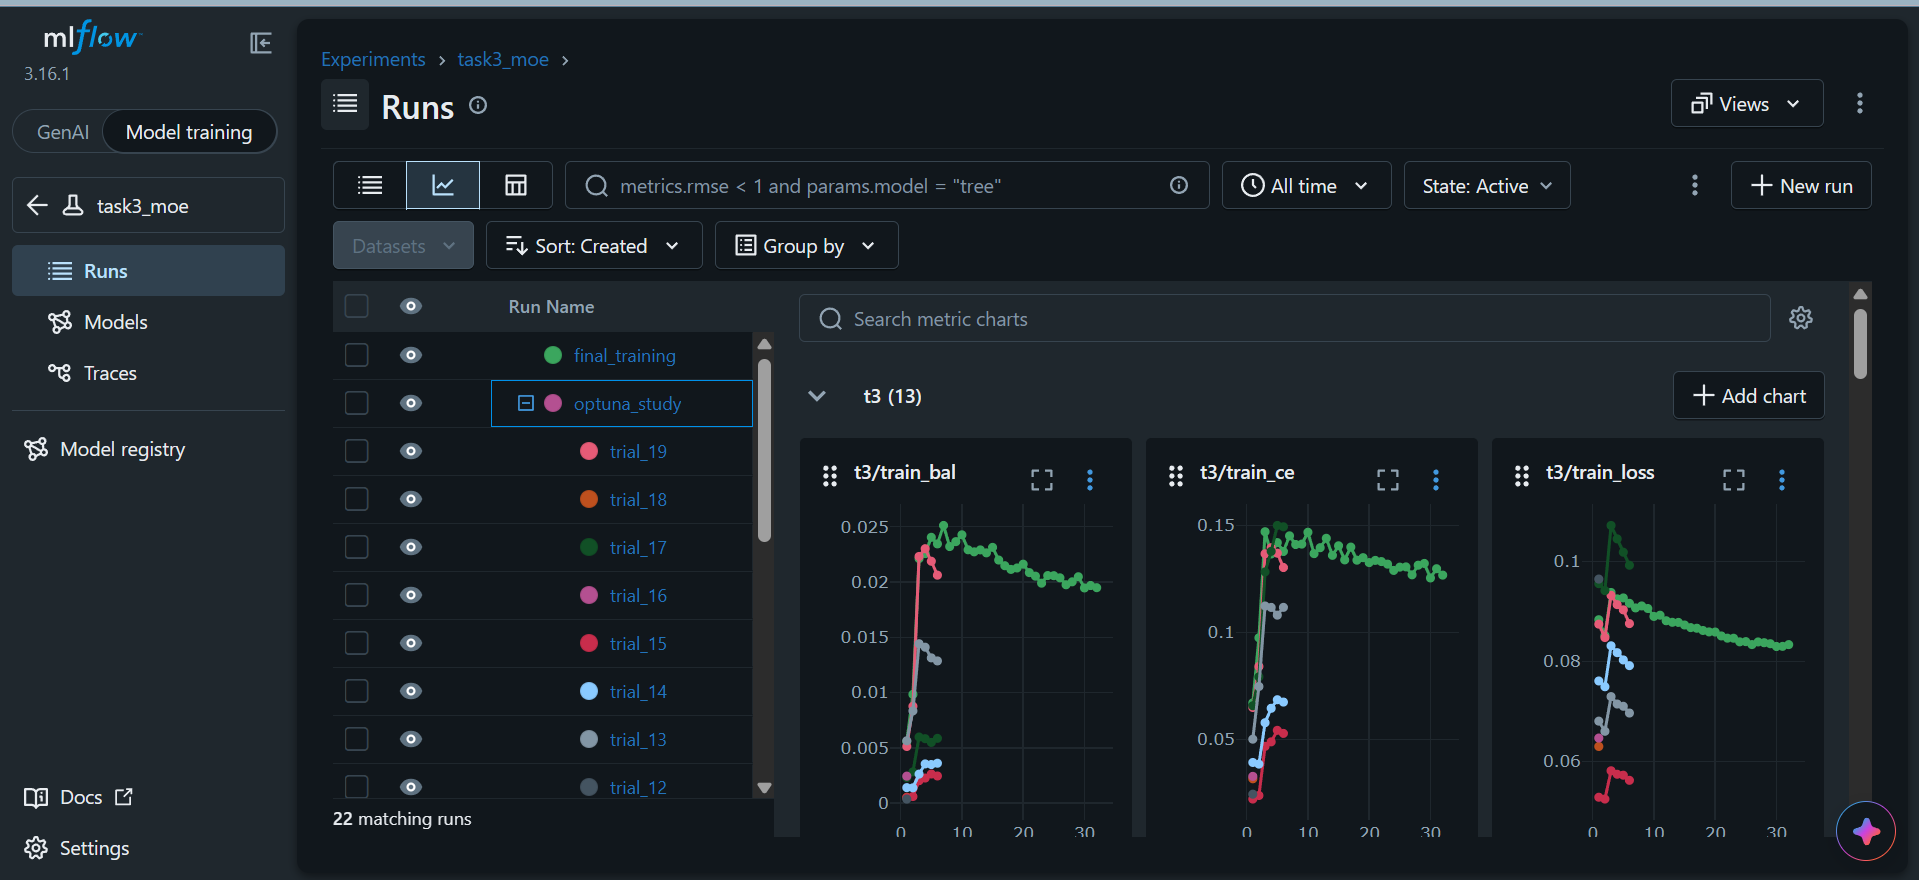
\includegraphics[width=0.49\textwidth]{figures/mlflow_t3.png}}{\fbox{\TODO{mlflow\_t3.png missing}}}\hfill
\IfFileExists{figures/mlflow_t4.png}{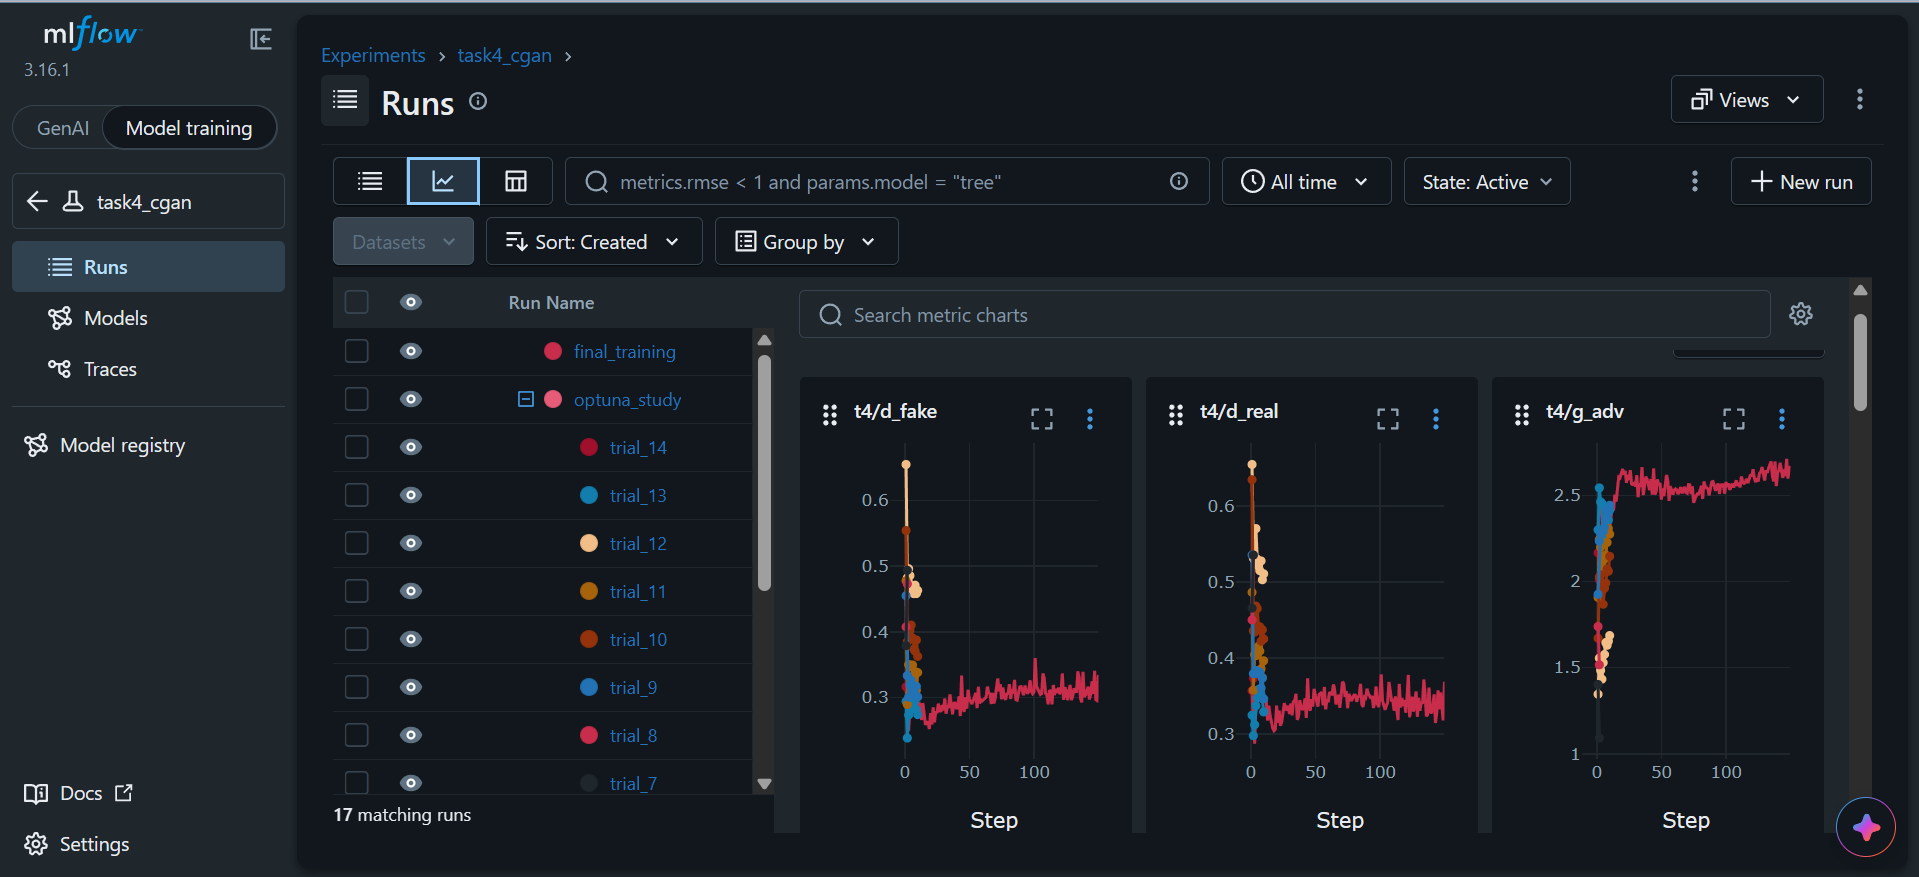
\includegraphics[width=0.49\textwidth]{figures/mlflow_t4.png}}{\fbox{\TODO{mlflow\_t4.png missing}}}
\caption{MLflow experiment tracking for each task (top left to bottom right: Task 1 UDAE, Task 2 classifier, Task 3 soft MoE, Task 4 cGAN). Each experiment holds a parent Optuna study with one nested run per trial, plus the final training run whose curves (the long line in each chart) are logged per epoch.}
\label{fig:mlflow}
\end{figure*}
\optfig{mlflow_experiments.png}{0.95\columnwidth}{MLflow experiment list: one experiment per training stage (Task 1, Task 2 classifier, Task 2 specialists, Task 3, Task 4).}{fig:mlflowexp}


% =============================================================================
\section{Results and Analysis}\label{sec:results}
\subsection{Task 1: universal autoencoder}
\gen{t1_by_type}
\gen{t1_by_level}
\optfigw{task1_examples.png}{0.95\textwidth}{Task 1: twelve test examples (clean target, corrupted input, reconstruction, absolute error).}{fig:t1ex}
\optfig{task1_failures.png}{0.95\columnwidth}{Task 1 failure cases (lowest PSNR).}{fig:t1fail}
\optfig{task1_curves.png}{0.95\columnwidth}{Task 1 training and validation curves.}{fig:t1curves}
\textbf{Analysis.} The UDAE removes salt-and-pepper noise well (PSNR $16.38\to24.76$\,dB, SSIM $0.412\to0.787$) and recovers occlusions partly ($13.61\to21.30$\,dB). It does not help with Gaussian blur. The blurred input already scores 27.78\,dB and the output scores 24.84\,dB, and SSIM also falls ($0.828\to0.780$). The twelve examples in Fig.~\ref{fig:t1ex} show the same thing in the error maps. For salt-and-pepper and blur the error is faint and spread over texture and edges, while for occlusion it is a bright block exactly where the black rectangles were, and the output there is a smooth guess. The training curves (Fig.~\ref{fig:t1curves}) fall steadily and flatten after about 45 epochs, with the validation objective ending near 0.27. The training loss sits at about half that value only because it is the $\alpha$-weighted loss and $\alpha\approx0.5$, not because the model generalises better than it should. The two curves never diverge, so I see no sign of overfitting and no reason to train longer.

The clean row explains why. The autoencoder reproduces a perfectly clean image only to 24.94\,dB, because the $8\times8$ bottleneck cannot store every detail. The outputs for salt-and-pepper (24.76) and blur (24.84) are within 0.2\,dB of this ceiling, so the denoising itself is essentially solved and what remains is the reconstruction loss of the architecture. Occlusion sits 3.6\,dB below the ceiling. That gap is real information loss: the pixels under the black rectangles are gone and the model can only paint a plausible guess. The error grows with the covered area (22.87, 21.41 and 19.60\,dB at low, medium and high severity). This is the main weakness of a bottleneck autoencoder judged by PSNR: it makes clean and blurred images worse. (The 100\,dB shown for clean images with the identity bypass is a capped value.)

Fig.~\ref{fig:t1fail} shows the four lowest-PSNR cases, and all four are the same test image, a cat on a large black background, under occlusion and salt-and-pepper noise. The outputs have a grey halo spreading from the cat into the background. So the failure comes from this image, since large flat dark regions are reproduced poorly, and not from the corruption type. I did not run an ablation to confirm the cause.

\subsection{Task 2: hard routing}
\gen{t2_classifier}
\gen{t2_routing}
\optfig{task2_confusion.png}{0.8\columnwidth}{Normalised confusion matrix of the corruption classifier on the test manifest.}{fig:cm}
\optfig{task2_misrouted.png}{0.95\columnwidth}{Cases where a classifier error breaks the restoration.}{fig:t2mis}
\optfig{task2_classifier_curves.png}{0.95\columnwidth}{Classifier training curves.}{fig:clscurves}
\optfig{task2_specialist_curves.png}{0.95\columnwidth}{Validation objective L1+(1-SSIM) of the three specialists during training.}{fig:speccurves}
\textbf{Analysis.} The classifier is almost perfect: accuracy 0.9989 and macro-F1 0.998 over 36{,}690 test entries. The clean class is the least reliable (precision 0.993, recall 0.995), which is expected, since a clean image is hardest to tell apart from a low-severity corruption. Only 42 entries (0.1\%) were misrouted, and the normalised confusion matrix (Fig.~\ref{fig:cm}) rounds to the identity, with every diagonal cell at 0.99 or 1.00. The classifier curves (Fig.~\ref{fig:clscurves}) show how easy the task is: validation accuracy is above 0.96 after two epochs and reaches about 0.99 after 20. There is one sharp dip to about 0.7 at epoch 7 that recovers by epoch 8; I did not investigate it, and it does not affect the final result. So oracle and predicted routing give the same PSNR on the corrupted classes to within 0.01\,dB. The only visible cost is on clean images, where the mean drops from 100 to 99.66\,dB because the few clean images sent to an expert come back at about 24\,dB instead of being copied exactly.

All four examples in Fig.~\ref{fig:t2mis} are clean images sent to the blur or occlusion expert. The blur expert softens them (23--25\,dB) and the occlusion expert paints a grey halo around a black background (9.7\,dB). So the cost of a routing error depends on which expert receives the image, and it is highest when a clean image goes to the occlusion expert.

The second finding is that the specialists do not beat the universal autoencoder. With oracle routing they average 23.33\,dB against 23.63\,dB for Task~1 (salt 24.63 versus 24.76, blur 24.36 versus 24.84, occlusion 21.00 versus 21.30). The specialists share one architecture chosen by a short search and each sees only a third of the corruption distribution, while the universal model trains for 60 epochs on everything. I did not run the ablation that would separate these causes. Like the universal model, the blur specialist ends below its input PSNR (24.36 versus 27.78\,dB). The specialist curves (Fig.~\ref{fig:speccurves}) agree with this. The salt-and-pepper and blur specialists end at nearly the same validation objective (about 0.26), the occlusion specialist stays much higher (about 0.37), and all three were still falling slowly at epoch 40, so longer training would probably have helped them.

\subsection{Task 3: soft mixture-of-experts}
\gen{t3_by_type}
\gen{t3_weights}
\gen{t3_health}
\gen{t3_mixed}
\gen{compare}
\optfigw{task3_examples.png}{0.95\textwidth}{Task 3: twelve test examples. The vector $w$ printed on the left is the gate weight for [identity, salt-and-pepper, blur, occlusion].}{fig:t3ex}
\optfig{task3_curves.png}{0.95\columnwidth}{Task 3 training and validation curves (joint stage).}{fig:t3curves}
\optfig{task3_routing_heatmap.png}{0.95\columnwidth}{Mean routing weights per test condition.}{fig:heat}
\optfig{task3_weight_distribution.png}{0.95\columnwidth}{Distribution of gate weights per true corruption type.}{fig:wdist}
\optfig{task3_dominant_vs_distributed.png}{0.95\columnwidth}{An example where one expert dominates (top) and one where weights are spread over several branches (bottom).}{fig:domdist}
\optfig{task3_mixed_corruption.png}{0.95\columnwidth}{Two simultaneous corruptions handled by the soft model.}{fig:mixed}
\optfig{task3_weight_evolution.png}{0.95\columnwidth}{Mean gate weights during warm-up (first epochs) and joint fine-tuning.}{fig:wevol}
\optfig{task3_failures.png}{0.95\columnwidth}{Task 3 failure cases with the gate weights $[w_0,w_1,w_2,w_3]$ printed on the left.}{fig:t3fail}
\textbf{Analysis.} The examples in Fig.~\ref{fig:t3ex} show how the gate behaves. Clean images get $w\approx[0.97\text{--}0.99,0,0,0.01\text{--}0.03]$ and a PSNR of about 55\,dB, so they pass through almost untouched. Salt-and-pepper images send 0.88--1.00 of the weight to the salt expert, and a high-severity blur image sends 0.97 to the blur expert. The occlusion examples are different: the occlusion expert gets only 0.64--0.79 and the identity branch keeps 0.21--0.35, so part of the black rectangle is copied through, and the error maps show the largest errors inside the rectangles (19.7\,dB at high severity). The validation curve in Fig.~\ref{fig:t3curves} falls from 0.206 to about 0.184 over the 32 epochs, a gain of roughly 11\%, and it is flat in the last ten epochs, so the fine-tuning helped but did not change the picture dramatically. The training loss is lower only because it is a weighted loss that is smaller than L1+(1-SSIM) by construction.

On single corruptions the soft MoE is the best system (Table~\ref{tab:compare}): 25.18, 25.62 and 21.84\,dB for salt-and-pepper, blur and occlusion, against 24.76, 24.84 and 21.30 for Task~1 and 24.63, 24.36 and 21.00 for oracle hard routing. The mean is 24.22\,dB against 23.63 and 23.33. This comparison is not perfectly fair. The MoE starts from the Task~2 weights and then trains for another 32 epochs, so it has seen more training than the other systems, and part of its gain may come from that.

On the mixed stress test the order reverses (Table~\ref{tab:t3_mixed}). The universal autoencoder reaches 19.42\,dB, the soft MoE 19.07\,dB and hard routing 18.88\,dB. Soft blending beats a hard choice (+0.19\,dB), but the gate was trained with one label per image, so it cannot pick two experts for two simultaneous corruptions, and the experts have never seen the second corruption. The three systems are within 0.55\,dB of each other, so routing gives no clear advantage here. Fig.~\ref{fig:mixed} shows why. In the blur plus salt-and-pepper examples the gate sends 0.98--0.99 to the salt expert and ignores the blur, so the dots are removed but the picture stays blurry. In the occlusion plus blur examples it sends 0.88--0.91 to the blur expert and none to the occlusion expert, so the black rectangles stay black and light up as the brightest regions of the error map. The gate picks one corruption and cannot select two experts, which is the limitation I expected from training on single labels.

On clean images the soft model scores 53.64\,dB instead of the 100\,dB of the hard identity bypass, because the identity branch gets a weight of about 0.95 and the experts leak the remaining 5\% (Table~\ref{tab:t3_w}). No branch is inactive or collapsed (Table~\ref{tab:t3_health}): the mean weights are 0.25, 0.28, 0.25 and 0.22, and each expert gets almost no weight on average on the wrong corruption type (at most 0.014; Fig.~\ref{fig:wdist} shows the same per image). The gate has also learned to blend by severity. The identity branch keeps a share of 0.37--0.38 for low-severity blur and occlusion and only 0.05--0.21 at high severity, while the expert weight rises with severity (blur 0.62, 0.89, 0.94; salt-and-pepper 0.87, 0.95, 0.97). Fig.~\ref{fig:heat} and Fig.~\ref{fig:wdist} summarise this routing. The box plots show that for clean and salt-and-pepper inputs the right branch gets a weight with a very narrow spread, while for blur and occlusion the spread is wide: the identity branch has a median of about 0.1 for blur and 0.27 for occlusion, with some images up to 0.6. Fig.~\ref{fig:domdist} contrasts a case where one expert dominates (a medium salt-and-pepper image with $w=[0,1.00,0,0]$) with a low-severity blur image where the gate hedges between three branches ($w=[0.40,0,0.40,0.19]$), which is what I would expect when the blur is barely visible. During joint training the batch-mean weights settled after about five epochs (Fig.~\ref{fig:wevol}). In that figure the identity branch averages about 0.37 because it is measured on class-balanced batches, while Table~\ref{tab:t3_health} averages over the test manifest, where only one entry in ten is clean, which is why it shows 0.25 there. I did not evaluate the gate on the test set before fine-tuning, so I cannot say how far fine-tuning moved it.

The failure cases (Fig.~\ref{fig:t3fail}) are the same black-background cat as in Task~1 (9.2 and 10.4\,dB, with correct routing at $w_{occ}=0.83$ and $0.74$) and high-severity salt-and-pepper images with saturated colours. There the green lawn comes back olive and the pink background beige even though the gate sends 0.87--0.98 of the weight to the right expert. So these failures are in the restoration and not in the routing.

\subsection{Task 4: face-to-sketch}
\gen{t4_results}
\optfigw{task4_examples.png}{0.8\textwidth}{Task 4: test photographs, ground-truth sketches and the three generated styles.}{fig:t4ex}
\optfig{task4_failures.png}{0.95\columnwidth}{Task 4 failure cases (highest L1).}{fig:t4fail}
\optfig{task4_gan_losses.png}{0.95\columnwidth}{Adversarial training losses.}{fig:ganloss}
\optfig{task4_l1_curves.png}{0.95\columnwidth}{Generator reconstruction loss and validation L1.}{fig:ganl1}
\optfig{task4_evolution.png}{0.95\columnwidth}{The same validation photographs rendered at fixed epoch intervals (rows: photograph, Style 1--3).}{fig:evolution}
\textbf{Analysis.} The cGAN is clearly better than the baseline of using the grayscale photo as the sketch (PSNR 15.61 versus 6.73\,dB, SSIM 0.538 versus 0.289, L1 0.106 versus 0.416). Results differ a lot by style. Style~2 is worst (12.34\,dB, L1 0.153) and Style~3 is best (18.66\,dB), but the test set has 619, 381 and only 46 images of the three styles, so the Style~3 number rests on very few samples. The Style~2 ground-truth sketches use dense dark hatching whose stroke positions cannot be predicted, so an L1-trained generator produces a smoother average and scores poorly even when the face is right.

The style condition is used by the model. With the correct style the L1 is 0.1056 and with a wrong style it is 0.1467, which is 39\% higher. Fig.~\ref{fig:t4ex} shows three distinct looks from the same photo: light thin lines for Style~1, heavy dark shading for Style~2 and a softer grey rendering for Style~3.

Training was stable (Fig.~\ref{fig:ganloss}). The discriminator losses stayed near 0.3 and the generator adversarial loss settled near 2.6 after about 20 epochs, above the equilibrium value of 0.69, so the discriminator stays ahead of the generator without overpowering it. Validation L1 fell from 0.118 to about 0.10 within 20 epochs and ended at 0.095 after 150 epochs, while the training reconstruction loss kept falling from 0.28 to 0.155 (Fig.~\ref{fig:ganl1}). The training value is probably higher because it is measured with augmentation and dropout switched on. Fig.~\ref{fig:evolution} shows the progress: after the first epochs the faces are smeared blobs, by the middle snapshots hair, eyes and mouth have lines, and in the last snapshots the three styles are clearly separate.

The highest-L1 failures (Fig.~\ref{fig:t4fail}) are all women with long dark or voluminous hair. The ground-truth hair is drawn with many strokes that the generator renders as lighter, smoother hair. Photos with reflective sunglasses also give a garbled eye region (last row of Fig.~\ref{fig:t4ex}).

% =============================================================================
\section{Application Architecture}\label{sec:app}
I made the interface design in Google Stitch from a written brief describing the page structure, colours, controls, cards and responsive layout (Fig.~\ref{fig:stitch}). I did this after the React and Tailwind CSS app was already working, so the design documents the interface and was not used as code. The Stitch screens show the same four workspaces as the app. The sample values on them (latency, PSNR, hardware name) are placeholder text generated by Stitch and are not results from this work. nginx serves the React bundle and proxies \texttt{/api} to a FastAPI container. The backend checks the file type and size, converts to RGB, resizes to $128\times128$, applies the requested corruption with the same code used in training, runs the ONNX models with ONNX Runtime and returns the images, the routing information and the timing. Fig.~\ref{fig:apparch} shows how the containers fit together and Fig.~\ref{fig:screens} shows the four workspaces in use, with the uploaded image, the corrupted input, the restored output and the routing information visible in each. The endpoints are \texttt{/api/health}, \texttt{/api/universal}, \texttt{/api/hard-route}, \texttt{/api/soft-moe} and \texttt{/api/face2sketch}. \texttt{docker compose up --build} starts everything at \texttt{http://localhost:8080}, with the ONNX files mounted from \texttt{./models}.
\optfig{arch_app.png}{0.95\columnwidth}{Deployment architecture.}{fig:apparch}
\optfigw{stitch_design.png}{0.95\textwidth}{Google Stitch design of the interface: design-system tokens and the four workspace screens (Universal Restoration, Hard-Routed Restoration, Soft Mixture-of-Experts, Face-to-Sketch Generator).}{fig:stitch}

\optfigw{app_screens.png}{0.95\textwidth}{Screenshots of the four workspaces: Universal Restoration, Hard-Routed Restoration, Soft Mixture-of-Experts Restoration and Face-to-Sketch Generator.}{fig:screens}


\subsection{ONNX export}
The universal autoencoder, the classifier, the three specialists, the full soft-MoE pipeline (gate, experts and temperature baked in) and the generator are exported with a dynamic batch axis. Table~\ref{tab:onnx} gives the largest absolute difference between PyTorch and ONNX Runtime outputs on random inputs.
\gen{onnx}

% =============================================================================
\section{Limitations}\label{sec:limits}
Occlusion removes information, so every model can only paint plausible content there. Pixel metrics understate the visual quality and also penalise other valid answers. PSNR, SSIM and L1 also favour blurry outputs, and I did not compute perceptual metrics such as LPIPS or FID.

The GAN Optuna objective measures fidelity to the paired sketch and not realism, and short trials may rank settings differently from full training. FS2K is small (about 900 training pairs after the split), and the photos of the three styles come from different sources, so style may be tied to image content. The Task~4 test set is also imbalanced across styles (619/381/46).

The classifier and experts are tuned for the four specified corruptions. Unseen degradations such as JPEG, motion blur or Gaussian noise are outside the training distribution, and I did not test any. For Gaussian blur, every bottleneck restorer ends below the PSNR of the blurred input (24.4--24.8 versus 27.8\,dB) and SSIM also drops, so by pixel metrics these models are worse than doing nothing on blur. A deblurring network with skip connections or a residual design would be needed. The Task~2 comparison between specialists and the universal model is not an ablation because the training budgets differ. Finally, everything runs at $128\times128$, and the app resizes larger uploads, which throws away detail.

\section{Conclusion}
The soft mixture-of-experts was the best strategy on single corruptions (mean 24.22\,dB against 23.63 for the universal autoencoder and 23.33 for hard routing), but the universal autoencoder was best when two corruptions were combined (19.42\,dB). Routing therefore helps only when the input matches what the experts were trained for. Classifying the corruption was not the bottleneck (99.9\% accuracy, oracle and predicted routing equal), and every bottleneck autoencoder failed on blur by ending below the PSNR of the blurred input. In the Optuna studies the loss weight $\alpha$ (autoencoders), regularisation (classifier), gate temperature and balance weight (MoE) and the two GAN learning rates mattered most, while network width and latent size mattered little. The style condition controls the cGAN output (L1 0.106 with the correct style against 0.147 with a wrong one), although fidelity is limited by the unpredictable strokes of Style~2 and the small Style~3 test set. With more time I would try a residual or skip-connection design for blur, train on mixed corruptions, run an ablation on specialist training budget, and add LPIPS for the GAN.

% =============================================================================
\appendices
\section{Use of AI Tools}
I used Claude (Anthropic) throughout this project. It wrote the first version of the code (data pipeline, model definitions, Optuna and MLflow scripts, ONNX export, FastAPI backend, React frontend and Docker files) and drafted the text of this report from my results. I ran all training on Google Colab, found and fixed the Colab and repository setup problems (the notebook clone and FS2K unzip steps, Git LFS and the folder layout), ran the Docker deployment and took the screenshots. The numbers in this report come from my own runs and result files. The generated code was checked with CPU smoke tests on synthetic data, PyTorch versus ONNX parity checks, API tests and a browser test. I also used Google Stitch to make the interface design in Fig.~\ref{fig:stitch}, after the React frontend already existed. No other AI tools were used.

\section{Reproducibility}
To reproduce the results, run \texttt{pip install -r requirements.txt}, then \texttt{bash scripts/run\_all.sh}, then \texttt{docker compose up --build}. The README in the repository lists the dataset download steps, the expected folder layout, the model download links and the demo workflow.

% =============================================================================
\begin{thebibliography}{99}
\bibitem{vincent2008} P.~Vincent, H.~Larochelle, Y.~Bengio and P.-A.~Manzagol, ``Extracting and composing robust features with denoising autoencoders,'' in \emph{Proc.\ ICML}, 2008.
\bibitem{zhang2017dncnn} K.~Zhang, W.~Zuo, Y.~Chen, D.~Meng and L.~Zhang, ``Beyond a Gaussian denoiser: Residual learning of deep CNN for image denoising,'' \emph{IEEE Trans.\ Image Process.}, vol.~26, no.~7, 2017.
\bibitem{pathak2016} D.~Pathak, P.~Kr\"ahenb\"uhl, J.~Donahue, T.~Darrell and A.~Efros, ``Context encoders: Feature learning by inpainting,'' in \emph{Proc.\ CVPR}, 2016.
\bibitem{li2022airnet} B.~Li, X.~Liu, P.~Hu, Z.~Wu, J.~Lv and X.~Peng, ``All-in-one image restoration for unknown corruption,'' in \emph{Proc.\ CVPR}, 2022.
\bibitem{wang2004ssim} Z.~Wang, A.~Bovik, H.~Sheikh and E.~Simoncelli, ``Image quality assessment: From error visibility to structural similarity,'' \emph{IEEE Trans.\ Image Process.}, vol.~13, no.~4, 2004.
\bibitem{jacobs1991} R.~Jacobs, M.~Jordan, S.~Nowlan and G.~Hinton, ``Adaptive mixtures of local experts,'' \emph{Neural Computation}, vol.~3, no.~1, 1991.
\bibitem{shazeer2017} N.~Shazeer \emph{et al.}, ``Outrageously large neural networks: The sparsely-gated mixture-of-experts layer,'' in \emph{Proc.\ ICLR}, 2017.
\bibitem{mirza2014} M.~Mirza and S.~Osindero, ``Conditional generative adversarial nets,'' arXiv:1411.1784, 2014.
\bibitem{isola2017} P.~Isola, J.-Y.~Zhu, T.~Zhou and A.~Efros, ``Image-to-image translation with conditional adversarial networks,'' in \emph{Proc.\ CVPR}, 2017.
\bibitem{ronneberger2015} O.~Ronneberger, P.~Fischer and T.~Brox, ``U-Net: Convolutional networks for biomedical image segmentation,'' in \emph{Proc.\ MICCAI}, 2015.
\bibitem{perez2018film} E.~Perez, F.~Strub, H.~de Vries, V.~Dumoulin and A.~Courville, ``FiLM: Visual reasoning with a general conditioning layer,'' in \emph{Proc.\ AAAI}, 2018.
\bibitem{ulyanov2016} D.~Ulyanov, A.~Vedaldi and V.~Lempitsky, ``Instance normalization: The missing ingredient for fast stylization,'' arXiv:1607.08022, 2016.
\bibitem{akiba2019} T.~Akiba, S.~Sano, T.~Yanase, T.~Ohta and M.~Koyama, ``Optuna: A next-generation hyperparameter optimization framework,'' in \emph{Proc.\ KDD}, 2019.
\bibitem{parkhi2012} O.~Parkhi, A.~Vedaldi, A.~Zisserman and C.~Jawahar, ``Cats and dogs,'' in \emph{Proc.\ CVPR}, 2012.
\bibitem{fan2022fs2k} D.-P.~Fan \emph{et al.}, ``Facial-sketch synthesis: A new challenge,'' \emph{Machine Intelligence Research}, vol.~19, 2022.
\end{thebibliography}

\end{document}
